\documentclass[12pt,letterpaper]{article}
\usepackage[utf8]{inputenc}
\usepackage[spanish, es-tabla]{babel}
\usepackage[version=3]{mhchem}
\usepackage[journal=jacs]{chemstyle}
\usepackage{amsmath}
\usepackage{amsfonts}
\usepackage{amssymb}
\usepackage{makeidx}
\usepackage{xcolor}
\usepackage[stable]{footmisc}
\usepackage[section]{placeins}
%Paquetes necesarios para tablas
\usepackage{longtable}
\usepackage{array}
\usepackage{xtab}
\usepackage{multirow}
\usepackage{colortab}
%Paquete para el manejo de las unidades
\usepackage{siunitx}
\sisetup{mode=text, output-decimal-marker = {,}, per-mode = symbol, qualifier-mode = phrase, qualifier-phrase = { de }, list-units = brackets, range-units = brackets, range-phrase = --}
\DeclareSIUnit[number-unit-product = \;] \atmosphere{atm}
\DeclareSIUnit[number-unit-product = \;] \pound{lb}
\DeclareSIUnit[number-unit-product = \;] \inch{"}
\DeclareSIUnit[number-unit-product = \;] \foot{ft}
\DeclareSIUnit[number-unit-product = \;] \yard{yd}
\DeclareSIUnit[number-unit-product = \;] \mile{mi}
\DeclareSIUnit[number-unit-product = \;] \pint{pt}
\DeclareSIUnit[number-unit-product = \;] \quart{qt}
\DeclareSIUnit[number-unit-product = \;] \flounce{fl-oz}
\DeclareSIUnit[number-unit-product = \;] \ounce{oz}
\DeclareSIUnit[number-unit-product = \;] \degreeFahrenheit{\SIUnitSymbolDegree F}
\DeclareSIUnit[number-unit-product = \;] \degreeRankine{\SIUnitSymbolDegree R}
\DeclareSIUnit[number-unit-product = \;] \usgallon{galón}
\DeclareSIUnit[number-unit-product = \;] \uma{uma}
\DeclareSIUnit[number-unit-product = \;] \ppm{ppm}
\DeclareSIUnit[number-unit-product = \;] \eqg{eq-g}
\DeclareSIUnit[number-unit-product = \;] \normal{\eqg\per\liter\of{solución}}
\DeclareSIUnit[number-unit-product = \;] \molal{\mole\per\kilo\gram\of{solvente}}
\usepackage{cancel}
%Paquetes necesarios para imágenes, pies de página, etc.
\usepackage{graphicx}
\usepackage{lmodern}
\usepackage{fancyhdr}
\usepackage[left=4cm,right=2cm,top=3cm,bottom=3cm]{geometry}

%Instrucción para evitar la indentación
%\setlength\parindent{0pt}
%Paquete para incluir la bibliografía
\usepackage[backend=bibtex,style=chem-acs,biblabel=dot]{biblatex}
\addbibresource{references.bib}

%Formato del título de las secciones

\usepackage{titlesec}
\usepackage{enumitem}
\titleformat*{\section}{\bfseries\large}
\titleformat*{\subsection}{\bfseries\normalsize}

%Creación del ambiente anexos
\usepackage{float}
\floatstyle{plaintop}
\newfloat{anexo}{thp}{anx}
\floatname{anexo}{Anexo}
\restylefloat{anexo}
\restylefloat{figure}

%Modificación del formato de los captions
\usepackage[margin=10pt,labelfont=bf]{caption}

%Paquete para incluir comentarios
\usepackage{todonotes}

%Paquete para incluir hipervínculos
\usepackage[colorlinks=true, 
            linkcolor = blue,
            urlcolor  = blue,
            citecolor = black,
            anchorcolor = blue]{hyperref}

%%%%%%%%%%%%%%%%%%%%%%
%Inicio del documento%
%%%%%%%%%%%%%%%%%%%%%%

\begin{document}
\renewcommand{\labelitemi}{$\checkmark$}

\renewcommand{\CancelColor}{\color{red}}

\newcolumntype{L}[1]{>{\raggedright\let\newline\\\arraybackslash}m{#1}}

\newcolumntype{C}[1]{>{\centering\let\newline\\\arraybackslash}m{#1}}

\newcolumntype{R}[1]{>{\raggedleft\let\newline\\\arraybackslash}m{#1}}

\begin{center}
	\textbf{\LARGE{Informe de Modulo 1}}\\
	\vspace{7mm}
		\textbf{\large{Solich, Ivan Exequiel}}\\
	\textbf{\large{Ortiz, Agustín}}\\
	\textbf{\large{Canteros, Francisco}}\\
	\vspace{4mm}
	\textbf{\large{Laboratorio de Calor y Termodinamica}}\\
	\textbf{\large{Grupo 7}}\\
	\textbf{\large{Profesor: }}\\
	\today
\end{center}

\vspace{7mm}

\section*{\centering Resumen}

El resumen es una versión condensada de todo el informe escrita en apenas 100 a 200 palabras. Para lograr este propósito el resumen debe contener una o dos frases introductorias al tema, la descripción del problema a resolver, el como fue resuelto, la metodología empleada, los principales resultados y/o conclusiones del trabajo. En la práctica es más fácil escribir el resumen al final, cuando las demás secciones estén listas.

\section{Introducción}

Esta sección debe incluir información general que explique la importancia del experimento. Se deben utilizar referencias para soportar la base científica del mismo; esto le da credibilidad, porque indica que preparó adecuadamente la práctica. Debe incluir la información relevante relacionada con los experimentos; haga especial énfasis en condiciones inusuales o críticas. Las referencias deben ir numeradas consecutivamente en el texto y aparecer como una lista en la sección~\nameref{sec:references}.\autocite{Cooper2009} Las referencias más comunes incluyen libros, manuales de laboratorio y artículos.

\section{Resultados}

En esta sección se debe presentar de forma condensada los datos obtenidos durante el experimento. Todos los datos deben ser resumidos en tablas y/o gráficas enumeradas. El título debe contener una descripción clara del contenido. 
Las tablas deben reservarse para reportar listas de valores, mientras que la relaciones entre variables deben reportarse en gráficas. Tanto las gráficas, los esquemas de reacción, las fotografías y las ilustraciones deben agruparse bajo el título figura. En la \ref{fig:esquema} se observa un ejemplo de un esquema de reacción.

\begin{figure}[h!]
\begin{floatrow}
\centering
\caption{Esquema de reacción}
\includegraphics[width=15cm]{./images/esquema.eps}
\label{fig:esquema}
\floatfoot{\small{FUENTE: Autor}}
\end{floatrow}
\end{figure}

\begin{longtable}{L{5cm}C{5cm}C{5cm}}
\caption{Papeles indicadores y cambios de pH. \autocite{Lozano2010}}
\label{tab:indicadorespH}\\
\hline
\bfseries{Papel Indicador} & \bfseries{Viraje de color} & \bfseries{Rango de pH}\\
\hline
\endfirsthead
\multicolumn{3}{c}{\bfseries \tablename{} \thetable \ldots continuación}\\
\hline
\bfseries{Papel Indicador} & \bfseries{Viraje de color} & \bfseries{Rango de pH}\\
\hline
\endhead
\hline
\multicolumn{3}{r}{\ldots continúa en la siguiente página}\\
\endfoot
\hline
\endlastfoot


\multirow{2}{*}{Papel tornasol neutro} & violeta $\rightarrow$ rojo & \num{7.0} -- \num{5.0} \\ 
& violeta $\rightarrow$ azul & \num{7.0} -- \num{8.0} \\ 
Papel tornasol azul & azul $\rightarrow$ rojo & \num{8.0} -- \num{5.0} \\ 
Papel tornasol rojo & rojo $\rightarrow$ azul & \num{5.0} -- \num{8.0} \\ 
Papel amarillo brillante & amarillo $\rightarrow$ rojo & \num{6.7} -- \num{7.9} \\ 
Papel Congo & azul $\rightarrow$ rojo & \num{8.0} -- \num{5.0} \\ 
Papel amarillo nitrazina & amarillo $\rightarrow$ violeta-azul & \num{6.0} -- \num{7.0} \\ 
Papel fenolftaleína & blanco $\rightarrow$ rojo & \num{8.3} -- \num{10.0} \\ 
\end{longtable}

\begin{figure}[h!]
\begin{floatrow}
\centering
\caption{Resultados del ensayo de insaturación}
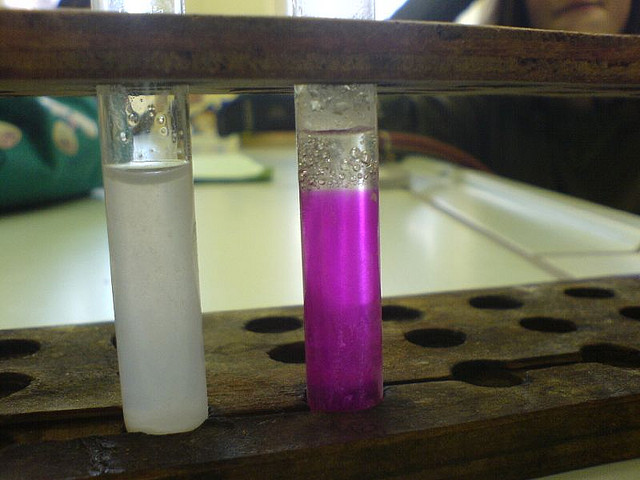
\includegraphics[width=10cm]{./images/tubes.jpg}
\label{fig:tubes}
\floatfoot{\small{FUENTE: flickr.com - bajo licencia creative commons}}
\end{floatrow}
\end{figure}

\begin{longtable}{C{3cm}C{4cm}C{4cm}C{4cm}}
\caption{Puntos de ebullición de las muestras problema.}
\label{tab:boiling}\\
\hline
\bfseries{Compuesto} & \bfseries{Punto de ebullición experimental \SI{}{\degreeCelsius}} & \bfseries{Punto de ebullición corregido \SI{}{\degreeCelsius}} & \bfseries{Punto de ebullición literatura \SI{}{\degreeCelsius}}\\
\hline
\endfirsthead
\multicolumn{2}{c}{\bfseries \tablename{} \thetable \ldots continuación}\\
\hline
\bfseries{Compuesto} & \bfseries{Punto de ebullición experimental \SI{}{\degreeCelsius}} & \bfseries{Punto de ebullición corregido \SI{}{\degreeCelsius}} & \bfseries{Punto de ebullición literatura \SI{}{\degreeCelsius}}\\
\hline
\endhead
\hline
\multicolumn{2}{r}{\ldots continúa en la siguiente página}\\
\endfoot
\hline
\endlastfoot

\includegraphics{./images/toluene.eps} & b & c & \num{110.6} \\ 
\includegraphics{./images/cyclohexane.eps} & b & c & \num{80.74} \\ 
\includegraphics{./images/cyclohexanol.eps} & b & \num{110.6} & \num{160.8} \\ \hline

\end{longtable}


\subsection{Muestra de cálculos}

\begin{equation}
E={ E }^{ 0 }-\frac { 0.05916 }{ 2 } \log _{ 10 }{ \frac { \frac { { \left[ { H }^{ + } \right]  }^{ 2 }{ F }_{ { H }_{ 2 }A } }{ { \left[ { H }^{ + } \right]  }^{ 2 }+{ \left[ { H }^{ + } \right]  }{ K }_{ 1 }+{ K }_{ 1 }{ K }_{ 2 } }  }{ { F }_{ D }{ \left[ { H }^{ + } \right]  }^{ 2 } }  } 
\end{equation}

\section{Discusión de Resultados\label{sec:discusion}}

\subsection{Corrección de los puntos de ebullición}

Los puntos de ebullición fueron corregidos utilizando la ecuación de Sydney-Young\autocite{young:1902} (Ecuación \ref{eq:bpcorrection}). En donde \textit{t} es el punto de ebullición experimental, $C = \dfrac{dP}{dt} \times \dfrac{1}{T}$ es un valor aproximadamente constante que puede aproximarse a \num{0.00012} para líquidos polares y a \num{0.00010} para líquidos no polares y \textit{p} es la presión atmosférica del laboratorio expresada en mmHg.

\begin{equation}
\label{eq:bpcorrection}
\Delta T = C(760 - p)(273 + t)
\end{equation}

Se encontraron desviaciones respecto a los valores experimentales reportados en la literatura como se observa en la \ref{tab:boiling}. La diferencia observada se le puede atribuir al menos a tres razones; primero la presión atmosférica del laboratorio en el momento del experimento no se pudo medir así que se tomó un valor de \SI{680}{\mmHg}. Segundo el termómetro que se utilizó no fue calibrado previamente además que era un termómetro de inmersión completa y en el experimento solo estaba sumergido el bulbo, por lo que no existe certeza sobre la exactitud de la medida. Finalmente, el valor hay que recordar que los valores de la constante \textit{C} son aproximados y que en realidad esta constante es diferente para cada líquido.

\subsection{Ecuaciones Químicas}

A continuación se muestra un ejemplo de una reacción química escrita con la ayuda del paquete \textit{mhchem}.

\begin{center}
\ce{1/2 O2 _{(g)} + 2 H+ + 2 e^- <=> H2O} \hspace{19mm} $\times 3$ \hspace{20mm} $E^0 = \SI{1.229}{\volt}$\\
\vspace{3mm}
\ce{2 Cr^{3+} + 7 H2O <=> Cr2O7^{2-} + 14 H+ + 6 e^-} \hspace{24mm} $E^0 = \SI{-1.36}{\volt}$\\
\underline{\hspace{145mm}}

\ce{3 O2 _{(g)} + 4 Cr^{3+} + 8 H2O <=> 2 Cr2O7^{2-} + 16 H+ } \hspace{15mm} $E^0 = \SI{-0.13}{\volt}$\\
\end{center}

\section{Conclusiones\label{sec:conclusions}}

\SI{0.100}{\Molar} \\



\SI{23}{\gram}\\

$\SI{10d-2}{\cancel\gram\of{\ce{Na2SO4}}} \times \dfrac{\SI{1}{\mole}}{\SI{80}{\cancel\gram\of{\ce{Na2SO4}}}} = $

\num{3.1415592d-3}

\begin{equation}
\label{eq:ensayo}
x=3y+5
\end{equation}

Ahora quiero referenciar la ecuación \ref{eq:ensayo} y continuo escribiendo

\ce{H2SO4 + Ca(OH)2 -> CaSO4 v + 2 H2O ^}

\begin{equation}
\label{eq:cuadratica}
x=\frac { -b\pm \sqrt [ 2 ]{ { b }^{ 2 }-4ac }  }{ 2a } 
\end{equation}

Si necesito referirme a la ecuación cuadrática (ver ecuación \ref{eq:cuadratica}) y continúo escribiendo


\section{Procedimiento Experimental\label{sec:procedure}}

\section{Referencias\label{sec:references}}


\printbibliography[heading=none]
		
\end{document}
